\documentclass[aspectratio=169,10pt]{beamer}

\usepackage[T1]{fontenc}
\usepackage[utf8]{inputenc}
\usepackage{lmodern}
\usepackage{microtype}
\usepackage{amsmath}
\usepackage{graphicx}
\usepackage{pgfplots}
\pgfplotsset{compat=1.18}
\usetikzlibrary{arrows.meta,positioning,calc}
\graphicspath{{../slides/}{../../thesis/assets/}{docs/slides/}}
% Generated by prepare_evidence.py from retained JSON; do not edit.
\newcommand{\FinalPrecision}{(1,57.142857) (2,100) (3,82.352941)}
\newcommand{\FinalRecall}{(1,66.666667) (2,83.333333) (3,77.777778)}
\newcommand{\FinalFone}{(1,61.538462) (2,90.909091) (3,80)}
\newcommand{\FinalTP}{(1,4) (2,10)}
\newcommand{\FinalFP}{(1,3) (2,0)}
\newcommand{\FinalFN}{(1,2) (2,2)}
\newcommand{\ProfileChromecast}{(1,5.4171533) (2,92.558367) (3,0.0043707875) (4,2.020109)}
\newcommand{\ProfileSamsung}{(1,36.565683) (2,0.16912304) (3,51.004054) (4,12.26114)}
\newcommand{\WindowDetected}{(10,38) (20,37) (30,45) (60,45)}
\newcommand{\WindowTimely}{(10,32) (20,17) (30,12) (60,6)}
\newcommand{\WindowFone}{(10,73.372781) (20,78.333333) (30,85.106383) (60,81.967213)}
\newcommand{\DelayChromecast}{(10,6.825) (20,13.466667) (30,16.991667) (60,36.933333)}
\newcommand{\DelaySamsung}{(10,5.2) (20,10.375) (30,17.766667) (60,30.933333)}
\newcommand{\Rejections}{(1,7) (2,5) (3,2)}
\newcommand{\BackendRatios}{(1,1.0644772) (2,1.1100044) (3,0.89920118)}
\newcommand{\EdgeMemory}{(0.0,67.082031) (2.5,68.054688) (5.0,68.28125) (7.5,68.414062) (10.0,68.835938) (12.5,68.835938) (15.0,68.835938) (17.5,68.917969) (20.0,68.917969)}
\newcommand{\EdgePeak}{68.92}
\newcommand{\EdgeWorst}{5.079}
\newcommand{\IncidentLabels}{S6,S5,S4,S3,S2,S1,C3,C2,C1}
\newcommand{\IncidentBars}{\draw[palerose,line width=5pt] (axis cs:0,1) -- (axis cs:10,1);
\draw[palerose,line width=5pt] (axis cs:0,2) -- (axis cs:10,2);
\draw[palerose,line width=5pt] (axis cs:0,3) -- (axis cs:10.0167,3);
\draw[palerose,line width=5pt] (axis cs:0,4) -- (axis cs:10,4);
\draw[palerose,line width=5pt] (axis cs:0,5) -- (axis cs:10,5);
\draw[palerose,line width=5pt] (axis cs:0,6) -- (axis cs:10.0167,6);
\draw[palerose,line width=5pt] (axis cs:0,7) -- (axis cs:10,7);
\draw[palerose,line width=5pt] (axis cs:0,8) -- (axis cs:10,8);
\node[anchor=west,font=\small,text=charcoal] at (axis cs:10.3,8) {missed};
\draw[palerose,line width=5pt] (axis cs:0,9) -- (axis cs:10.0167,9);}
\newcommand{\IncidentAlerts}{(8.833333333333334,1) (5.5,2) (12.183333333333334,3) (6.116666666666666,4) (2.783333333333333,5) (9.466666666666667,6) (9.2,7) (4.616666666666666,9)}


% Visual system retained from docs/slides/lm_idnet_project_presentation.tex.
\definecolor{burgundy}{HTML}{990000}
\definecolor{darkburgundy}{HTML}{59000E}
\definecolor{dustyrose}{HTML}{D1545B}
\definecolor{palerose}{HTML}{E5D5D6}
\definecolor{paper}{HTML}{F7F6F2}
\definecolor{softgray}{HTML}{ECEAE7}
\definecolor{midgray}{HTML}{77736F}
\definecolor{charcoal}{HTML}{434343}
\definecolor{ink}{HTML}{111111}
\setbeamercolor{normal text}{fg=ink,bg=paper}
\setbeamercolor{structure}{fg=burgundy}
\setbeamercolor{frametitle}{fg=ink,bg=paper}
\setbeamercolor{block title}{fg=white,bg=darkburgundy}
\setbeamercolor{block body}{fg=ink,bg=softgray}
\setbeamercolor{takeaway}{fg=darkburgundy,bg=palerose!65!paper}
\setbeamerfont{normal text}{size=\large}
\setbeamerfont{frametitle}{series=\bfseries,size=\Large}
\setbeamerfont{block title}{series=\bfseries,size=\normalsize}
\setbeamersize{text margin left=.65cm,text margin right=.65cm}
\hyphenpenalty=10000
\exhyphenpenalty=10000
\setbeamertemplate{navigation symbols}{}
\setbeamertemplate{itemize item}{\color{burgundy}$\blacktriangleright$}
\AddToHook{shipout/foreground}{%
  \begin{tikzpicture}[remember picture,overlay]
    \node[anchor=north west,inner sep=0pt]
      at ([xshift=.12cm,yshift=-.10cm]current page.north west)
      {\ifnum\value{page}=1\relax
         
\includegraphics[height=.82cm,decodearray={1 0 1 0 1 0}]{unipd-seal.png}%
       \else
         \ifnum\value{page}=10\relax
           
\includegraphics[height=.82cm,decodearray={1 0 1 0 1 0}]{unipd-seal.png}%
         \else
           \includegraphics[height=.76cm]{unipd_logo.png}%
         \fi
       \fi};
    \ifnum\value{page}=1\relax
      \node[anchor=north east,inner sep=0pt]
        at ([xshift=.61\paperwidth,yshift=-.10cm]current page.north west)
        {
\includegraphics[height=.68cm,decodearray={1 0 1 0 1 0}]{dei_logo.png}};
    \else
      \ifnum\value{page}=10\relax
        \node[anchor=north east,inner sep=0pt]
          at ([xshift=.61\paperwidth,yshift=-.10cm]current page.north west)
          {
\includegraphics[height=.68cm,decodearray={1 0 1 0 1 0}]{dei_logo.png}};
      \else
        \node[anchor=north east,inner sep=0pt]
          at ([xshift=-.12cm,yshift=-.10cm]current page.north east)
          {
\includegraphics[height=.66cm]{dei_logo.png}};
      \fi
    \fi
  \end{tikzpicture}%
}
\setbeamertemplate{frametitle}{%
  \vspace{.18cm}\hspace*{.30cm}\insertframetitle\par\vspace{-.1cm}%
  {\color{burgundy}\rule{\textwidth}{.6pt}}%
}
\newcommand{\slideprefix}{}
\newcommand{\slidetotal}{/10}
\setbeamertemplate{footline}{%
  \hbox{%
    \begin{beamercolorbox}[wd=.83\paperwidth,ht=2.8ex,dp=1.1ex,leftskip=1em]{author in head/foot}%
      \color{charcoal}\scriptsize LM-IDNet\quad\textbullet\quad\insertsectionhead
    \end{beamercolorbox}%
    \begin{beamercolorbox}[wd=.17\paperwidth,ht=2.8ex,dp=1.1ex,rightskip=1em]{date in head/foot}%
      \hfill\color{burgundy}\scriptsize\slideprefix\insertframenumber\slidetotal
    \end{beamercolorbox}%
  }%
}
\newcommand{\takeaway}[1]{%
  \vfill\begin{beamercolorbox}[sep=.16cm,wd=\textwidth]{takeaway}%
    \normalsize\bfseries #1
  \end{beamercolorbox}}
\newcommand{\evidence}[1]{\par\vspace{.09cm}{\fontsize{8}{9}\selectfont\color{charcoal}#1\par}}
\newcommand{\bigvalue}[1]{{\color{burgundy}\fontsize{29}{31}\selectfont\bfseries #1}}
\tikzset{
  flowbox/.style={draw=burgundy,line width=.8pt,rounded corners=1pt,
    fill=paper,minimum height=1cm,text width=2.6cm,align=center,font=\normalsize},
  lightbox/.style={flowbox,draw=charcoal,fill=softgray},
  flowarrow/.style={-{Latex[length=2.3mm]},thick,draw=charcoal}
}
\pgfplotsset{discussion/.style={
  axis lines=left,axis line style={charcoal},tick style={draw=none},
  tick label style={font=\small,text=ink},label style={font=\small,text=ink},
  title style={font=\normalsize\bfseries,text=ink},
  ymajorgrids=true,grid style={softgray},
  legend style={draw=none,fill=paper,font=\small,cells={anchor=west}},
  every axis plot/.append style={line width=1.4pt},
  clip=false,
},values/.style={nodes near coords,point meta=y,
  every node near coord/.append style={font=\small,text=ink,
    /pgf/number format/fixed,/pgf/number format/precision=1}}}

\title{LM-IDNet: Adaptive IoT Network Anomaly Detection}
\subtitle{Dirichlet--Multinomial Anomaly Detection for IoT Traffic}
\author{Fatemeh Mahvari}
\institute{Supervisor: Professor Mauro Migliardi\\Co-supervisor: Professor Alessandro Languasco}
\date{}
\hypersetup{pdftitle={LM-IDNet: Adaptive IoT Network Anomaly Detection},
  pdfauthor={Fatemeh Mahvari},pdfsubject={12-minute presentation with reference slides}}
\pdfstringdefDisableCommands{\def\translate#1{#1}}

\begin{document}

% 01 | 00:00–00:45 | 45 seconds
\begin{frame}[plain]
\begin{tikzpicture}[remember picture,overlay]
  \fill[ink] (current page.south west) rectangle (current page.north east);
  \fill[darkburgundy] (current page.south west) rectangle
    ([xshift=.64\paperwidth]current page.north west);
  \fill[burgundy,opacity=.28] ([xshift=.58\paperwidth]current page.south west)
    rectangle ([xshift=.67\paperwidth]current page.north west);
  \node[anchor=east,inner sep=0pt] (detector)
    at ([xshift=-.42cm]current page.east)
    {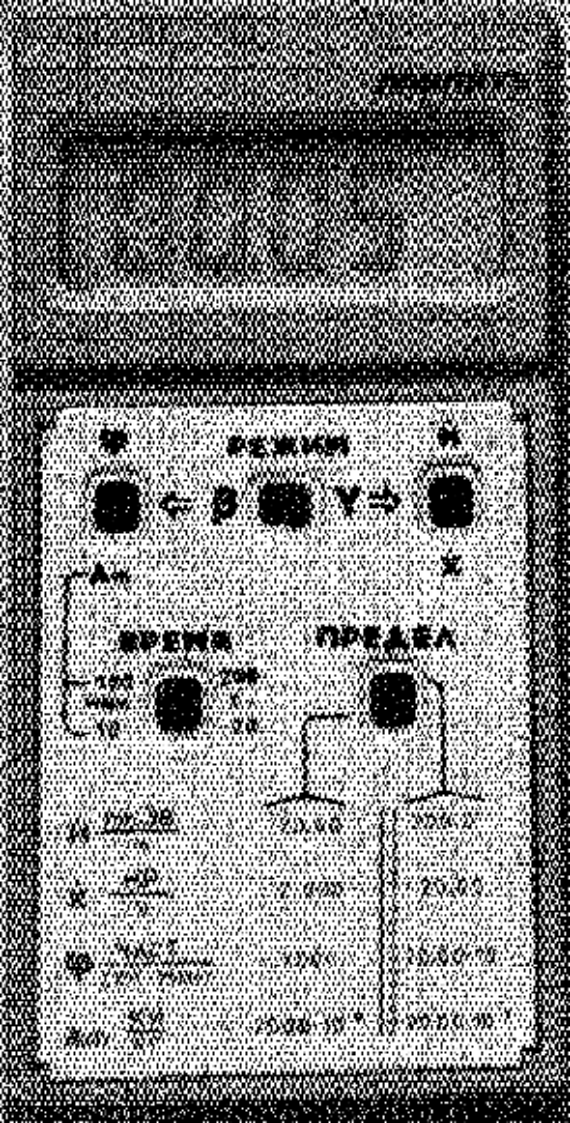
\includegraphics[height=.91\paperheight]{anomaly_detector.png}};
  \draw[palerose,line width=.8pt]
    ([xshift=-.10cm,yshift=.10cm]detector.north west) rectangle
    ([xshift=.10cm,yshift=-.10cm]detector.south east);
  \node[anchor=west,text width=.52\paperwidth]
    at ([xshift=.72cm,yshift=1.25cm]current page.west)
    {\color{white}\large\bfseries LM-IDNet: Adaptive IoT Network\\Anomaly Detection};
  \node[anchor=north,align=center,text width=.38\paperwidth]
    at ([xshift=.31\paperwidth,yshift=-.24cm]current page.north west)
    {\color{palerose}\scriptsize Department of Information Engineering};
  \node[anchor=west,text width=.50\paperwidth]
    at ([xshift=.72cm,yshift=-1.15cm]current page.west)
    {\color{white}\normalsize\bfseries Dirichlet--multinomial anomaly detection\\
     \color{palerose}\small Languasco--Migliardi likelihood evaluation};
  \node[anchor=south west,text width=.53\paperwidth]
    at ([xshift=.72cm,yshift=.30cm]current page.south west)
    {\color{palerose}\scriptsize Master's Degree in Computer Engineering\\[.08cm]
     \color{white}\small\bfseries Fatemeh Mahvari\quad\textbullet\quad Student ID: 2141994\\
     \color{palerose}\scriptsize Supervisor: Professor Mauro Migliardi\\
     Co-supervisor: Professor Alessandro Languasco\\
     Scientific support: Professor Sherenaz Al-Haj Baddar\\
     Academic Year 2025/2026};
  \node[anchor=south east,fill=ink,inner sep=2pt]
    at ([xshift=-.06cm,yshift=.06cm]detector.south east)
    {\color{palerose}\fontsize{6}{7}\selectfont REFERENCE IMAGE / PRYPIAT DETECTOR};
\end{tikzpicture}
\end{frame}

\section{System}

% 02 | 00:45–01:45 | 60 seconds
\begin{frame}{Context: IoT anomaly-detection approaches}
\begin{columns}[T,onlytextwidth]
\column{.31\textwidth}
\begin{block}{Research studies}
\small N-BaIoT, Kitsune and D\"IoT use richer neural, ensemble or federated representations.
\end{block}
\small Strong modelling capacity, but different data and protocols prevent a direct metric ranking.
\column{.31\textwidth}
\begin{block}{Operational platforms}
\small Agentless discovery, broad telemetry, threat intelligence and SOC response.
\end{block}
\small Microsoft Defender for IoT and Palo Alto Device Security address a wider operational scope.
\column{.31\textwidth}
\begin{block}{Scope of this study}
\small Four explicit counts, a device-specific normal model and inspectable decision margins.
\end{block}
\small Dirichlet--multinomial scoring, numerical validation and a constrained-runtime evaluation.
\end{columns}
\takeaway{LM-IDNet proposes device-specific detection from four counts using a Dirichlet--multinomial (DM) model.}
\evidence{It combines composition, traffic-volume and ARP checks with calibrated margins and guarded periodic refitting.}
\end{frame}

% 03 | 01:45–03:00 | 75 seconds
\begin{frame}{Four counts, three signals, one explainable decision}
\centering
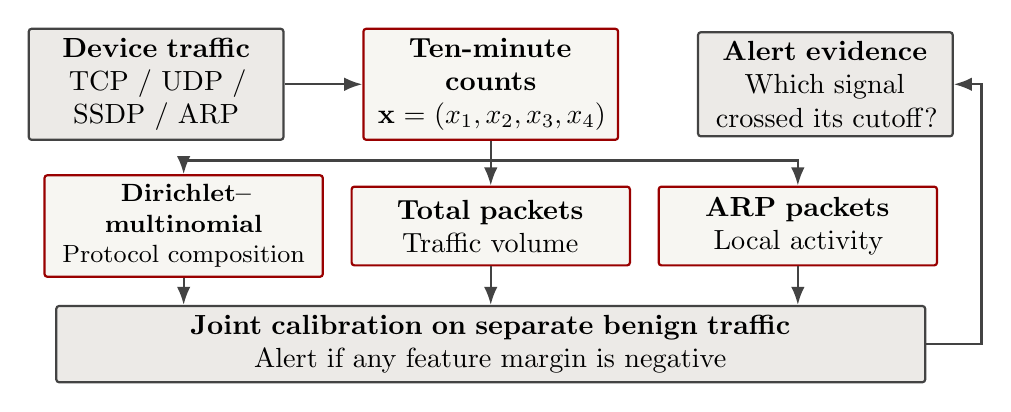
\begin{tikzpicture}[node distance=.45cm]
  \node[lightbox,text width=3cm] (input) at (-4.25,0)
    {\textbf{Device traffic}\\TCP / UDP / SSDP / ARP};
  \node[flowbox,text width=3cm] (counts) at (0,0)
    {\textbf{Ten-minute counts}\\$\mathbf{x}=(x_1,x_2,x_3,x_4)$};
  \node[lightbox,text width=3cm] (output) at (4.25,0)
    {\textbf{Alert evidence}\\Which signal\\crossed its cutoff?};
  \draw[flowarrow] (input) -- (counts);
  \node[flowbox,text width=3.3cm,font=\small] (dm) at (-3.9,-1.8)
    {\textbf{Dirichlet--multinomial}\\Protocol composition};
  \node[flowbox,text width=3.3cm] (volume) at (0,-1.8)
    {\textbf{Total packets}\\Traffic volume};
  \node[flowbox,text width=3.3cm] (arp) at (3.9,-1.8)
    {\textbf{ARP packets}\\Local activity};
  \draw[flowarrow] (counts.south) -- ++(0,-.25) -| (dm.north);
  \draw[flowarrow] (counts.south) -- (volume.north);
  \draw[flowarrow] (counts.south) -- ++(0,-.25) -| (arp.north);
  \node[lightbox,text width=10.8cm,minimum height=.8cm] (cal) at (0,-3.3)
    {\textbf{Joint calibration on separate benign traffic}\\
     Alert if any feature margin is negative};
  \draw[flowarrow] (dm.south) -- (dm.south |- cal.north);
  \draw[flowarrow] (volume.south) -- (cal.north);
  \draw[flowarrow] (arp.south) -- (arp.south |- cal.north);
  \draw[flowarrow] (cal.east) -- ++(.7,0) |- (output.east);
\end{tikzpicture}
\takeaway{The Languasco--Migliardi (LM) algorithm evaluates the DM likelihood using stable log-gamma differences.}
\evidence{Concentration measures how tightly traffic stays around its average protocol mix; $\psi$ is its inverse. A smaller $\psi$ is closer to the multinomial limit, where direct log-gamma subtraction can lose precision.}
\end{frame}

\section{Evaluation}

% 04 | 03:00–04:00 | 60 seconds
\begin{frame}{Datasets and chronological partitions}
\centering
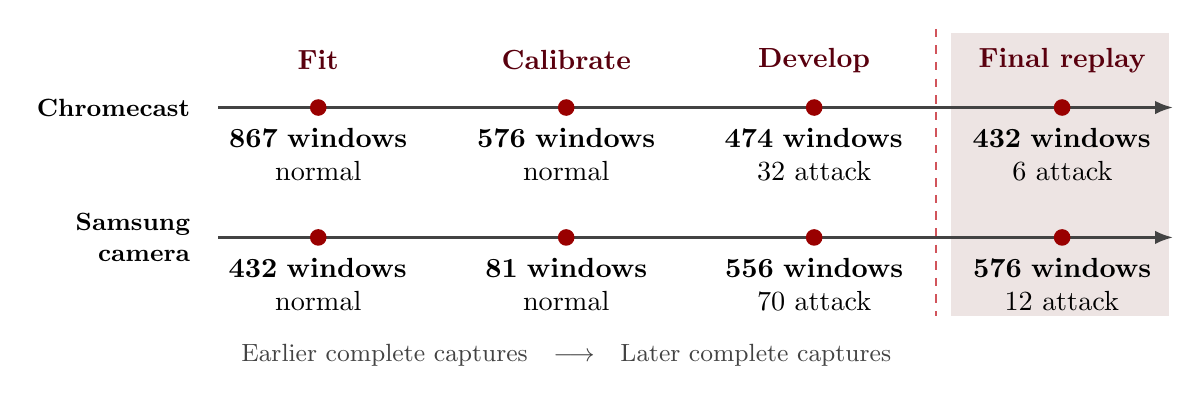
\begin{tikzpicture}[x=.94cm]
  \fill[palerose!55!paper] (8.55,.95) rectangle (11.5,-2.65);
  \foreach \x/\label in {0/Fit,3.35/Calibrate,6.7/Develop,10.05/Final replay}{
    \node[font=\normalsize\bfseries,text=darkburgundy] at (\x,.6) {\label};
  }
  \node[anchor=east,font=\small\bfseries] at (-1.6,0) {Chromecast};
  \node[anchor=east,font=\small\bfseries,align=right] at (-1.6,-1.65) {Samsung\\camera};
  \draw[flowarrow,line width=1pt] (-1.35,0) -- (11.55,0);
  \draw[flowarrow,line width=1pt] (-1.35,-1.65) -- (11.55,-1.65);
  \foreach \x/\n/\detail in {0/867/normal,3.35/576/normal,6.7/474/32 attack,10.05/432/6 attack}{
    \fill[burgundy] (\x,0) circle (3pt);
    \node[font=\normalsize,align=center,text width=2.35cm] at (\x,-.6)
      {\textbf{\n{} windows}\\\detail};
  }
  \foreach \x/\n/\detail in {0/432/normal,3.35/81/normal,6.7/556/70 attack,10.05/576/12 attack}{
    \fill[burgundy] (\x,-1.65) circle (3pt);
    \node[font=\normalsize,align=center,text width=2.35cm] at (\x,-2.25)
      {\textbf{\n{} windows}\\\detail};
  }
  \draw[dustyrose,dashed,thick] (8.35,1) -- (8.35,-2.65);
  \node[font=\small,align=center,text=charcoal] at (3.35,-3.15)
    {Earlier complete captures\quad$\longrightarrow$\quad Later complete captures};
\end{tikzpicture}
\takeaway{ICNC 2025 ALM baseline: $\psi<0.05$; Chromecast passes, Samsung does not.}
\evidence{Reference: Al-Haj Baddar, Languasco and Migliardi. Values: $0.0356$ / $0.0575$; both show extra-multinomial variation. Labels are used only for metrics.}
\end{frame}

% 05 | 04:00–05:25 | 85 seconds
\begin{frame}{Numerical comparison: LM and SciPy}
\begin{columns}[c,onlytextwidth]
\column{.63\textwidth}
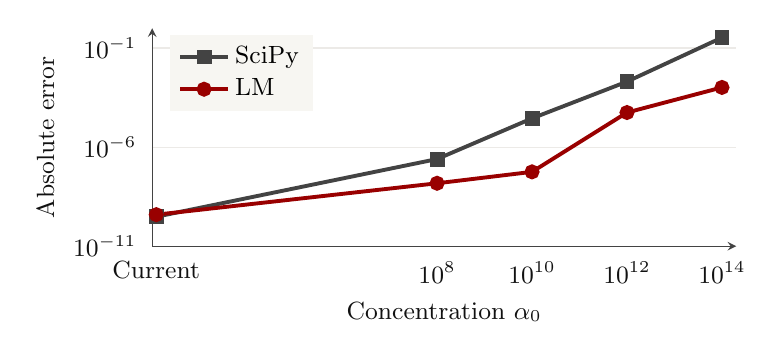
\begin{tikzpicture}
\begin{axis}[discussion,width=9.0cm,height=4.35cm,
  xmode=log,ymode=log,xmin=100,xmax=2e14,ymin=1e-11,ymax=1,
  xtick={122.22,1e8,1e10,1e12,1e14},
  xticklabels={Current,$10^8$,$10^{10}$,$10^{12}$,$10^{14}$},
  xlabel={Concentration $\alpha_0$},ylabel={Absolute error},
  legend style={at={(.03,.97)},anchor=north west}]
  \addplot[color=charcoal,mark=square*] coordinates {
    (122.22,3.07e-10) (1e8,2.50e-7) (1e10,2.83e-5)
    (1e12,2.02e-3) (1e14,3.37e-1)};
  \addplot[color=burgundy,mark=*] coordinates {
    (122.22,3.91e-10) (1e8,1.50e-8) (1e10,5.65e-8)
    (1e12,5.58e-5) (1e14,1.03e-3)};
  \legend{SciPy,LM}
\end{axis}
\end{tikzpicture}
\column{.33\textwidth}
\bigvalue{$\sim$500$\times$}\par
\small lower absolute error at $\alpha_0=10^{10}$\par\medskip
\bigvalue{$\sim$327$\times$}\par
\small lower absolute error at $\alpha_0=10^{14}$\par\medskip
{\color{charcoal}\small Current data: 0/1300 decision differences.}
\end{columns}
\vspace{-.08cm}
\fontsize{7.4}{8.2}\selectfont
\textbf{Live score:} LM 12.04 $\mu$s vs SciPy 13.39 $\mu$s (10.1\% faster).\quad
\textbf{Fit/refit:} LM 193 ms vs SciPy 181 ms (LM 6.4\% slower).
\takeaway{Both agree on current data; LM has lower error in the high-concentration stress regime.}
\evidence{100-digit reference probe. Runtime is workload-specific; ten-minute collection dominates alert delay.}
\end{frame}
% 06 | 05:25–07:10 | 105 seconds
\begin{frame}{Final detection results by device}
\centering
\normalsize Ten-minute windows\quad\textbullet\quad Final partitions
\vspace{.15cm}
\begin{columns}[c,onlytextwidth]
\column{.49\textwidth}
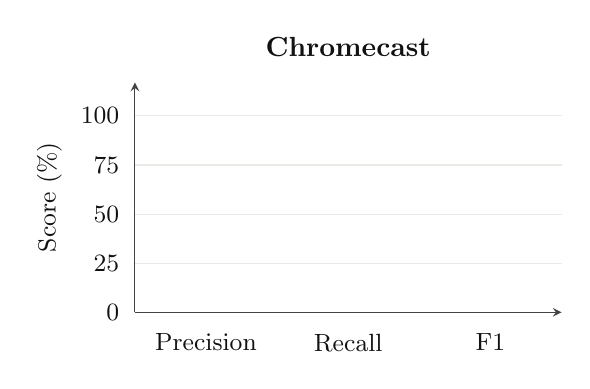
\begin{tikzpicture}
\begin{axis}[discussion,width=7cm,height=4.5cm,ybar,bar width=18pt,
  title={Chromecast},
  ymin=0,ymax=117,ytick={0,25,50,75,100},ylabel={Score (\%)},
  xmin=.5,xmax=3.5,xtick={1,2,3},xticklabels={Precision,Recall,F1}]
  \addplot[fill=charcoal,draw=charcoal,values] coordinates {\FinalStaticChromecast};
  \addplot[fill=burgundy,draw=burgundy,values] coordinates {\FinalPeriodicChromecast};
\end{axis}
\end{tikzpicture}
\column{.49\textwidth}
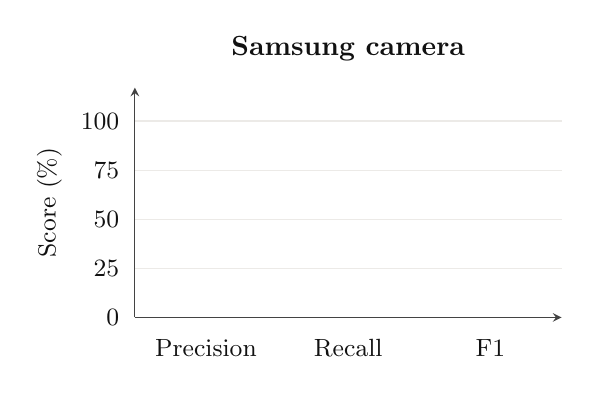
\begin{tikzpicture}
\begin{axis}[discussion,width=7cm,height=4.5cm,ybar,bar width=18pt,
  title={Samsung camera},
  ymin=0,ymax=117,ytick={0,25,50,75,100},ylabel={Score (\%)},
  xmin=.5,xmax=3.5,xtick={1,2,3},xticklabels={Precision,Recall,F1}]
  \addplot[fill=charcoal,draw=charcoal,values] coordinates {\FinalStaticSamsung};
  \addplot[fill=burgundy,draw=burgundy,values] coordinates {\FinalPeriodicSamsung};
\end{axis}
\end{tikzpicture}
\end{columns}
\small\textcolor{charcoal}{\rule{.35cm}{.16cm}}\ Static\qquad
\textcolor{burgundy}{\rule{.35cm}{.16cm}}\ Conservative periodic refit
\takeaway{Chromecast: 4/6 attack windows flagged. Samsung camera: 10/12 flagged.}
\evidence{Periodic-refit results match static results for each device; no candidate update was activated.}
\end{frame}

% 07 | 07:10–08:25 | 75 seconds
\begin{frame}{Attack coverage and detection delay}
\begin{columns}[c,onlytextwidth]
\column{.66\textwidth}
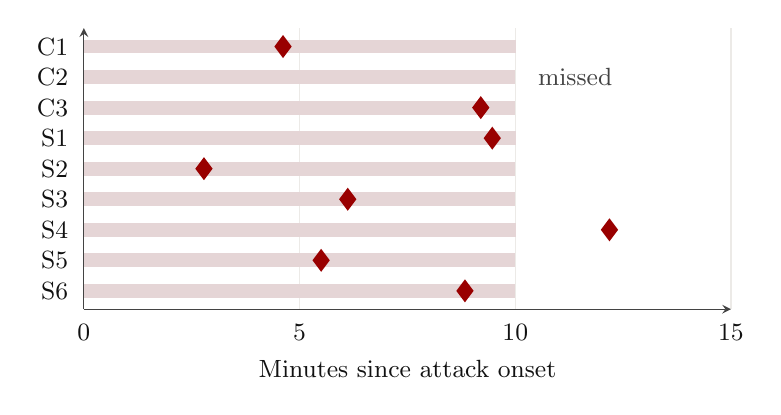
\begin{tikzpicture}
\begin{axis}[discussion,width=9.8cm,height=5.15cm,
  xmin=0,xmax=15,ymin=.4,ymax=9.6,xtick={0,5,10,15},
  ytick={1,2,3,4,5,6,7,8,9},yticklabels/.expanded={\IncidentLabels},
  xlabel={Minutes since attack onset},ymajorgrids=false,xmajorgrids=true,
  grid style={softgray}]
  \IncidentBars
  \addplot[only marks,mark=diamond*,mark size=3pt,color=burgundy]
    coordinates {\IncidentAlerts};
\end{axis}
\end{tikzpicture}
\column{.30\textwidth}
\textcolor{burgundy}{$\blacklozenge$}\ \textbf{First alert}\\
\textcolor{palerose}{\rule{.5cm}{4pt}}\ Annotated attack\par\bigskip
\textbf{Chromecast}\\2/3 detected; 2/3 by end\\
\bigvalue{6.9}\ min median\par\medskip
\textbf{Samsung camera}\\6/6 detected; 5/6 by end\\
\bigvalue{7.5}\ min median
\end{columns}
\takeaway{The ten-minute collection interval is part of the detection delay.}
\evidence{Static mode, final official intervals; C = Chromecast, S = Samsung. Median delay is among detected attacks; alerts occur at window close.}
\end{frame}

\section{Summary and limits}

% 08 | 08:25–09:30 | 65 seconds
\begin{frame}{Edge architecture and simulation}
\centering
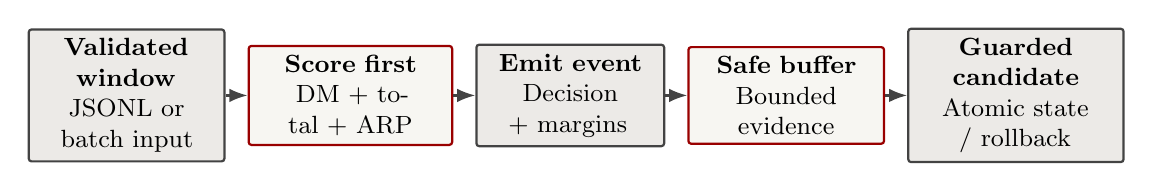
\begin{tikzpicture}[node distance=.28cm]
  \node[lightbox,text width=2.25cm,font=\small] (input)
    {\textbf{Validated window}\\JSONL or batch input};
  \node[flowbox,text width=2.35cm,font=\small,right=of input] (score)
    {\textbf{Score first}\\DM + total + ARP};
  \node[lightbox,text width=2.15cm,font=\small,right=of score] (event)
    {\textbf{Emit event}\\Decision + margins};
  \node[flowbox,text width=2.25cm,font=\small,right=of event] (buffer)
    {\textbf{Safe buffer}\\Bounded evidence};
  \node[lightbox,text width=2.5cm,font=\small,right=of buffer] (state)
    {\textbf{Guarded candidate}\\Atomic state / rollback};
  \draw[flowarrow] (input) -- (score);
  \draw[flowarrow] (score) -- (event);
  \draw[flowarrow] (event) -- (buffer);
  \draw[flowarrow] (buffer) -- (state);
\end{tikzpicture}
\vspace{-.04cm}
\begin{columns}[c,onlytextwidth]
\column{.62\textwidth}
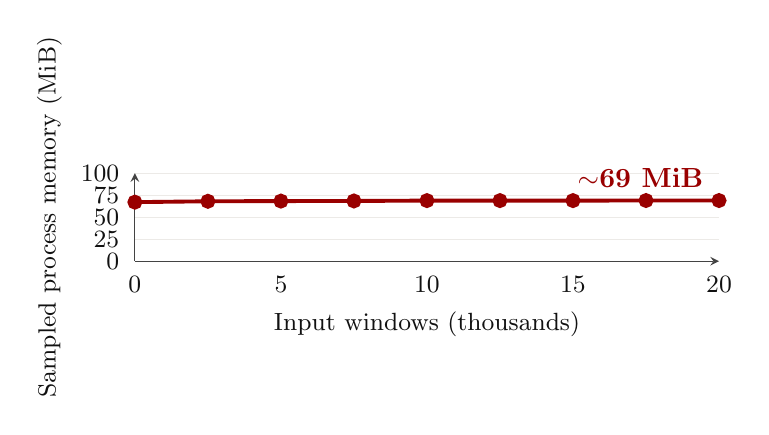
\begin{tikzpicture}
\begin{axis}[discussion,width=9.0cm,height=2.7cm,
  xmin=0,xmax=20,ymin=0,ymax=100,ytick={0,25,50,75,100},
  xtick={0,5,10,15,20},xlabel={Input windows (thousands)},
  ylabel={Sampled process memory (MiB)}]
  \addplot[color=burgundy,mark=*,mark size=2pt] coordinates {\EdgeMemory};
  \node[anchor=south east,font=\normalsize\bfseries,text=burgundy]
    at (axis cs:19.8,73) {$\sim$69 MiB};
\end{axis}
\end{tikzpicture}
\column{.34\textwidth}
\raggedright
\bigvalue{20,000}\par
\small inputs: 16,000 scored; 4,000 missing skipped\par
\bigvalue{$\sim$69 MiB}\par
\small sampled process memory\par
{\small\textbf{5.079 s} worst observed window, including a rejected refit}
\end{columns}
\vspace{-.18cm}
\takeaway{One detector serves batch and streaming; updates affect only later windows.}
\evidence{Accelerated synthetic replay; x86\_64 Docker, 1 CPU / 512 MiB. No candidate update was promoted.}
\end{frame}

% 09 | 09:30–10:25 | 55 seconds
\begin{frame}{Summary: results and limitations}
\begin{columns}[T,onlytextwidth]
\column{.48\textwidth}
\begin{block}{Observed results}
\small
\begin{itemize}
  \item Four counts support three inspectable alert signals.
  \item 8/9 attack intervals were alerted; 7 by attack end.
  \item LM reduces absolute error in the high-concentration stress regime.
  \item Streaming remained near 69 MiB with guarded persistent state.
\end{itemize}
\end{block}
\column{.48\textwidth}
\begin{block}{Scope and limitations}
\small
\begin{itemize}
  \item Two labelled devices and 18 final attack windows.
  \item Count-preserving attacks may remain invisible.
  \item The edge trial is synthetic x86\_64, not a physical gateway.
  \item Useful conservative adaptation remains unproven on these traces.
\end{itemize}
\end{block}
\end{columns}
\takeaway{The prototype combines explainable detection, stable likelihood evaluation and guarded runtime state.}
\evidence{Claims remain limited to the recorded datasets, numerical probe and constrained simulation.}
\end{frame}

% 10 | 10:25–10:40 | 15 seconds
\begin{frame}[plain,label=thanks]
\begin{tikzpicture}[remember picture,overlay]
  \fill[darkburgundy] (current page.south west) rectangle (current page.north east);
  \fill[ink] ([xshift=.76\paperwidth]current page.south west) rectangle (current page.north east);
  \node[anchor=west] at ([xshift=1cm,yshift=.9cm]current page.west)
    {\color{white}\fontsize{34}{38}\selectfont\bfseries Thank you};
  \node[anchor=west,text width=10cm] at ([xshift=1cm,yshift=-.3cm]current page.west)
    {\color{palerose}\Large Questions and discussion};
  \node[anchor=south west,text width=12cm] at ([xshift=1cm,yshift=.7cm]current page.south west)
    {\color{white}\normalsize LM-IDNet\quad\textbullet\quad Fatemeh Mahvari\\[.18cm]
     \color{palerose}\small Reference slides follow: model, profiles, native method, counts, guards, window study, sources.};
\end{tikzpicture}
\end{frame}

\appendix
\setcounter{framenumber}{0}
\renewcommand{\slideprefix}{R}
\renewcommand{\slidetotal}{}
\section{Reference / questions only}

\begin{frame}[label=reference-model]{R1 / Model and decision rule}
\normalsize
\textbf{DM composition model}\quad$\alpha_k>0$, $\alpha_0=\sum_k\alpha_k$, $N=\sum_kx_k$
\[
\ell(\mathbf{x})=\log\frac{N!}{\prod_kx_k!}
+\log\frac{\Gamma(\alpha_0)}{\Gamma(\alpha_0+N)}
+\sum_k\log\frac{\Gamma(\alpha_k+x_k)}{\Gamma(\alpha_k)}.
\]
\textbf{Three signals}\quad$\ell(\mathbf{x})$, $-\log(1+N)$, $-\log(1+x_{\mathrm{ARP}})$.
\par\medskip
Fit-only medians and IQRs scale each signal. The minimum scaled signal is
calibrated jointly at the 1\% lower quantile on separate benign windows.
\par\medskip
The event score is the minimum signed margin from the resulting cutoffs:
\[
s=\min(m_{\mathrm{DM}},m_N,m_{\mathrm{ARP}}),\qquad
\text{alert if }s<0,\qquad\text{severity}=\max(0,-s).
\]
\takeaway{During updates, original DM and count references remain active detection checks.}
\evidence{Constant fit features use unit scale. A count-tail breach can decide early. Severity is not an attack probability.}
\end{frame}

\begin{frame}[label=reference-profiles]{R2 / Device traffic profiles}
\begin{columns}[c,onlytextwidth]
\column{.62\textwidth}
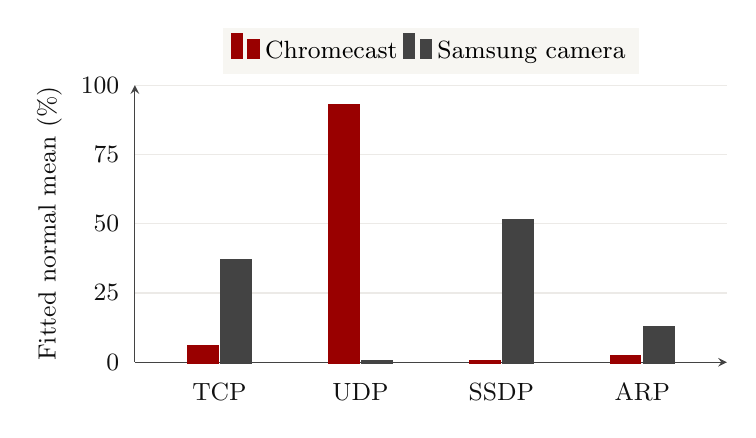
\begin{tikzpicture}
\begin{axis}[discussion,width=9.1cm,height=5.1cm,ybar,bar width=10pt,
  ymin=0,ymax=100,ytick={0,25,50,75,100},xmin=.4,xmax=4.6,
  xtick={1,2,3,4},xticklabels={TCP,UDP,SSDP,ARP},
  ylabel={Fitted normal mean (\%)},
  legend style={at={(.5,1.04)},anchor=south},legend columns=2]
  \addplot[fill=burgundy,draw=burgundy] coordinates {\ProfileChromecast};
  \addplot[fill=charcoal,draw=charcoal] coordinates {\ProfileSamsung};
  \legend{Chromecast,Samsung camera}
\end{axis}
\end{tikzpicture}
\column{.34\textwidth}
{\large\bfseries Device-specific models}\par\medskip
Normal protocol proportions differ between devices.\par\bigskip
\textbf{4 exclusive counts}\\per ten-minute window\par\medskip
Learn from a trusted benign period; flag unusual later behaviour.
\end{columns}
\takeaway{A separate normal model captures each device's traffic pattern.}
\evidence{Fitted means from saved normal-only models. UDP excludes SSDP; bars are model expectations.}
\end{frame}

\begin{frame}[label=reference-backend]{R3 / Native Languasco--Migliardi implementation}
\begin{columns}[c,onlytextwidth]
\column{.49\textwidth}
\begin{tikzpicture}
\begin{axis}[discussion,width=7cm,height=4.5cm,ybar,bar width=32pt,
  title={Complete fitting},xmin=.5,xmax=1.5,ymin=0,ymax=240,
  ytick={0,50,100,150,200},xtick={1},xticklabels={846 $\times$ 4 fit matrix},
  ylabel={Time (milliseconds)}]
  \addplot[fill=burgundy,draw=burgundy,values] coordinates {(1,\LmFit)};
\end{axis}
\end{tikzpicture}
\column{.49\textwidth}
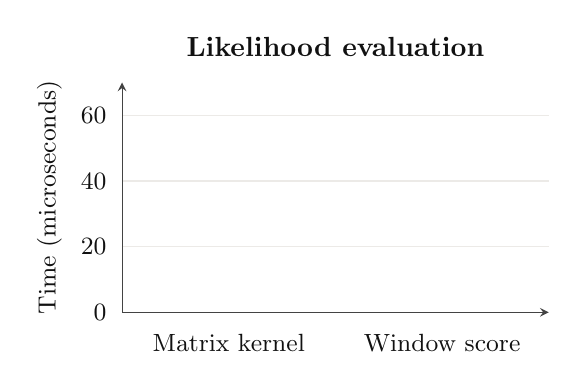
\begin{tikzpicture}
\begin{axis}[discussion,width=7cm,height=4.5cm,ybar,bar width=27pt,
  title={Likelihood evaluation},xmin=.5,xmax=2.5,ymin=0,ymax=70,
  ytick={0,20,40,60},xtick={1,2},xticklabels={Matrix kernel,Window score},
  ylabel={Time (microseconds)}]
  \addplot[fill=burgundy,draw=burgundy,values] coordinates {\LmKernelTimes};
\end{axis}
\end{tikzpicture}
\end{columns}
\takeaway{Native integration preserves the sum of independent window likelihoods.}
\evidence{Retained D-Link native-method timings, five batches and warm-up. Fitting excludes input/output. These are recorded measurements.}
\end{frame}

\begin{frame}[label=reference-counts]{R4 / Final confusion counts by device}
\begin{columns}[c,onlytextwidth]
\column{.63\textwidth}
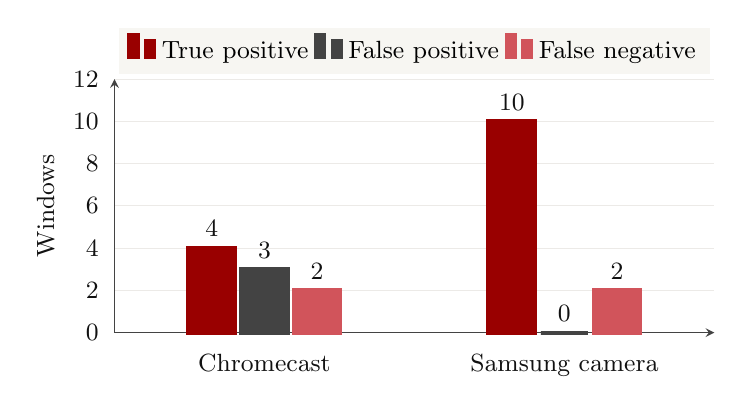
\begin{tikzpicture}
\begin{axis}[discussion,width=9.2cm,height=4.8cm,ybar,bar width=17pt,
  xmin=.5,xmax=2.5,ymin=0,ymax=12,ytick={0,2,4,6,8,10,12},
  xtick={1,2},xticklabels={Chromecast,Samsung camera},ylabel={Windows},
  legend style={at={(.5,1.02)},anchor=south},legend columns=3]
  \addplot[fill=burgundy,draw=burgundy,values] coordinates {\FinalTP};
  \addplot[fill=charcoal,draw=charcoal,values] coordinates {\FinalFP};
  \addplot[fill=dustyrose,draw=dustyrose,values] coordinates {\FinalFN};
  \legend{True positive,False positive,False negative}
\end{axis}
\end{tikzpicture}
\column{.33\textwidth}
\textbf{Chromecast}\\432 windows; 6 attack\\TP = 4\quad FP = 3\\FN = 2\quad TN = 423\\FPR = 3/426 = 0.70\%\par\medskip
\textbf{Samsung camera}\\576 windows; 12 attack\\TP = 10\quad FP = 0\\FN = 2\quad TN = 564\\FPR = 0/564 = 0\%
\end{columns}
\takeaway{Window recall and attack-interval coverage answer different questions.}
\evidence{Static mode, final partitions. A window is attack-labelled if it overlaps an official attack interval.}
\end{frame}

\begin{frame}[label=reference-guards]{R5 / Conservative learning guards}
\centering
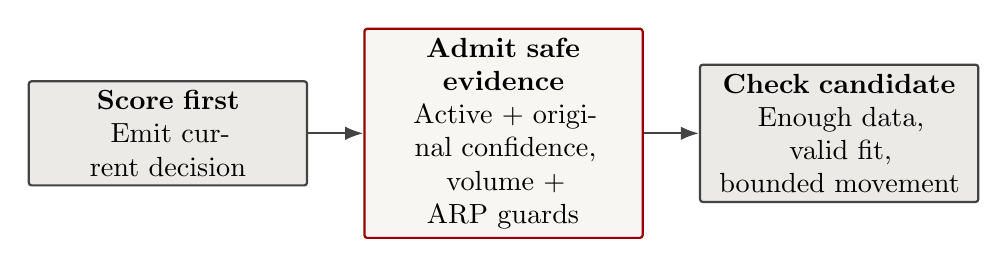
\begin{tikzpicture}
  \node[lightbox,text width=3.3cm] (score) {\textbf{Score first}\\Emit current decision};
  \node[flowbox,text width=3.3cm,right=.7cm of score] (admit)
    {\textbf{Admit safe evidence}\\Active + original confidence,\\volume + ARP guards};
  \node[lightbox,text width=3.3cm,right=.7cm of admit] (fit)
    {\textbf{Check candidate}\\Enough data, valid fit,\\bounded movement};
  \draw[flowarrow] (score) -- (admit);\draw[flowarrow] (admit) -- (fit);
\end{tikzpicture}
\vspace{.2cm}
\begin{align*}
  1/1.25\;&\leq\alpha'_0/\alpha_{0,t}\leq1.25
    &&\text{concentration ratio}\\[.12cm]
  \max_k|p'_k-p_{k,t}|\;&\leq0.05
    &&\text{protocol proportions}\\[.12cm]
  |\tau'-\tau_t|\;&\leq2\,\mathrm{IQR}_0
    &&\text{threshold movement}
\end{align*}
\normalsize Defaults: 288-window buffer; attempt every 144 scored windows;
144 accepted windows required for periodic fitting.
\takeaway{Rejecting a candidate retains the complete active pair; accepted pairs support rollback.}
\evidence{Per-update guards do not establish immunity to stealthy attacks or unlimited cumulative drift. Final replay promoted no candidates.}
\end{frame}

\begin{frame}[label=reference-coverage]{R6 / Window duration: attack coverage}
\begin{columns}[c,onlytextwidth]
\column{.49\textwidth}
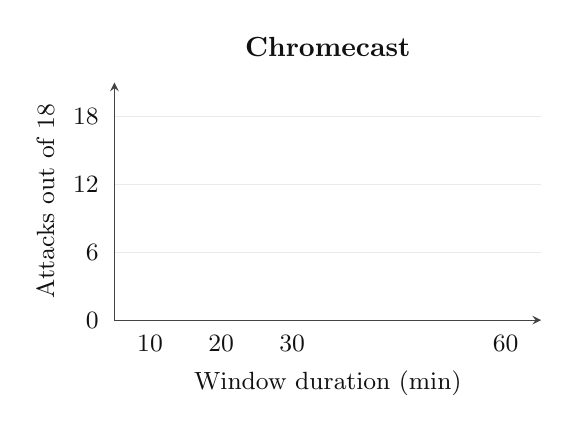
\begin{tikzpicture}
\begin{axis}[discussion,width=7cm,height=4.6cm,
  title={Chromecast},xmin=5,xmax=65,ymin=0,ymax=21,
  xtick={10,20,30,60},ytick={0,6,12,18},
  xlabel={Window duration (min)},ylabel={Attacks out of 18}]
  \addplot[color=burgundy,mark=*,values] coordinates {\WindowDetectedChromecast};
  \addplot[color=charcoal,dashed,mark=square*,values,
    every node near coord/.append style={anchor=west,xshift=3pt,yshift=1pt,
      fill=paper,inner sep=1pt}] coordinates {\WindowTimelyChromecast};
\end{axis}
\end{tikzpicture}
\column{.49\textwidth}
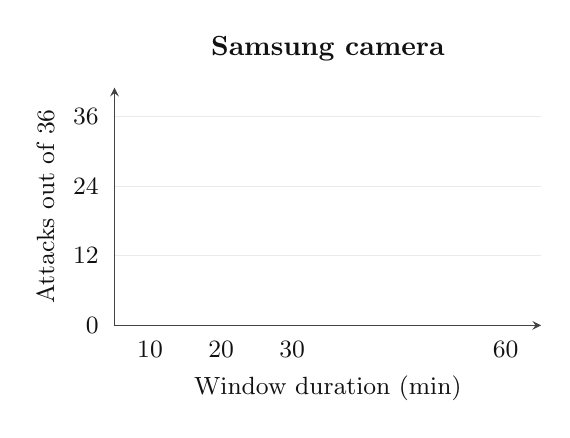
\begin{tikzpicture}
\begin{axis}[discussion,width=7cm,height=4.6cm,
  title={Samsung camera},xmin=5,xmax=65,ymin=0,ymax=41,
  xtick={10,20,30,60},ytick={0,12,24,36},
  xlabel={Window duration (min)},ylabel={Attacks out of 36}]
  \addplot[color=burgundy,mark=*,values] coordinates {\WindowDetectedSamsung};
  \addplot[color=charcoal,dashed,mark=square*,values,
    every node near coord/.append style={anchor=west,xshift=3pt,yshift=1pt,
      fill=paper,inner sep=1pt}] coordinates {\WindowTimelySamsung};
\end{axis}
\end{tikzpicture}
\end{columns}
\centering\small\textcolor{burgundy}{$\bullet$}\ Detected\qquad
\textcolor{charcoal}{$\blacksquare$}\ Alerted by attack end
\takeaway{Delivered reference: ten minutes. Longer windows increase response delay.}
\evidence{Static development study; matched traffic within each device; fresh fitting and calibration at every duration.}
\end{frame}

\begin{frame}[label=reference-duration]{R7 / Window duration: F1 and detection delay}
\begin{columns}[c,onlytextwidth]
\column{.49\textwidth}
\begin{tikzpicture}
\begin{axis}[discussion,width=7.0cm,height=4.6cm,
  title={Static window F1},xmin=5,xmax=65,ymin=0,ymax=105,
  xtick={10,20,30,60},ytick={0,25,50,75,100},
  xlabel={Window duration (min)},ylabel={F1 (\%)},
  legend style={at={(.03,.03)},anchor=south west,font=\small}]
  \addplot[color=burgundy,mark=*,values,
    every node near coord/.append style={anchor=north,yshift=-3pt}]
    coordinates {\WindowFoneChromecast};
  \addplot[color=charcoal,dashed,mark=square*,values] coordinates {\WindowFoneSamsung};
  \legend{Chromecast,Samsung}
\end{axis}
\end{tikzpicture}
\column{.49\textwidth}
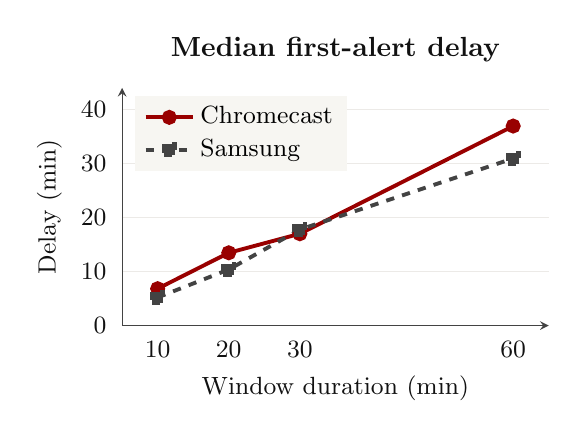
\begin{tikzpicture}
\begin{axis}[discussion,width=7.0cm,height=4.6cm,
  title={Median first-alert delay},xmin=5,xmax=65,ymin=0,ymax=44,
  xtick={10,20,30,60},ytick={0,10,20,30,40},
  xlabel={Window duration (min)},ylabel={Delay (min)},
  legend style={at={(.03,.97)},anchor=north west,font=\small}]
  \addplot[color=burgundy,mark=*] coordinates {\DelayChromecast};
  \addplot[color=charcoal,dashed,mark=square*] coordinates {\DelaySamsung};
  \legend{Chromecast,Samsung}
\end{axis}
\end{tikzpicture}
\end{columns}
\takeaway{F1 changes with label granularity; median delay is conditional on detection.}
\evidence{Static development study. Samsung uses May 28--29 to fit and May 30--31 to calibrate at every duration. Lines join measured settings.}
\end{frame}

\begin{frame}[label=reference-sources]{R8 / References and project evidence}
\small
\textbf{Statistical learning}\par\smallskip
Minka, \emph{Estimating a Dirichlet distribution}, 2000 / revised 2012.\\
Fixed-point estimation of the DM parameters.
\par\medskip
\textbf{Native likelihood method}\par\smallskip
Languasco and Migliardi, \emph{Computational Statistics} 38, 2023.\\
\href{https://doi.org/10.1007/s00180-022-01311-7}{doi: 10.1007/s00180-022-01311-7}\\
Al-Haj Baddar, Languasco and Migliardi, \emph{ICNC}, 2025.\\
\href{https://doi.org/10.1109/ICNC64010.2025.10993688}{doi: 10.1109/ICNC64010.2025.10993688}\\
Al-Haj Baddar, Languasco and Migliardi, \emph{IEEE TPAMI} 47(2), 2025.\\
\href{https://doi.org/10.1109/TPAMI.2024.3489645}{doi: 10.1109/TPAMI.2024.3489645}
\par\medskip
\textbf{Research and market context}\par\smallskip
N-BaIoT, Kitsune and D\"IoT: neural, ensemble and federated research systems.\\
Microsoft Defender for IoT and Palo Alto Device Security: representative commercial scope.
\par\smallskip
\textbf{Project evidence}\par\smallskip
Source code, protocols, results and reproducibility records:\\
\href{https://github.com/Pitclair/iot_anomaly_detection}
  {\texttt{github.com/Pitclair/iot\_anomaly\_detection}}
\end{frame}

\end{document}
